\documentclass[12pt,a4paper,oneside]{report}
\usepackage[english]{babel}
\selectlanguage{english}
\usepackage[T1]{fontenc}
\usepackage{times}
\usepackage[utf8]{inputenc}
\usepackage{amsmath}

\usepackage{graphicx}
\usepackage{multicol}
\usepackage{multirow}
\usepackage{longtable}
\usepackage{tabularx} % Para tablas de mas de una página
\usepackage{booktabs} 

\usepackage{nicematrix}

\usepackage{verbatim}

\usepackage{calc}
\usepackage[refpages]{gloss}
\usepackage{float}
\usepackage{anysize}
\usepackage{bigstrut}
\usepackage{appendix}
%\usepackage{lscape} 
\usepackage{pdflscape}
\usepackage{listings}
\usepackage{color}
\usepackage{setspace}
\usepackage{enumerate} 
\usepackage{ragged2e}
\usepackage[utf8]{inputenc}
\usepackage{comment}
\usepackage{pslatex}
\usepackage{apacite} 
\usepackage{fixltx2e}
\usepackage{caption}
\usepackage{setspace} 
\captionsetup[table]{skip=10pt}
\usepackage{array}

%%%%%%%% Probando referencias
%\usepackage[a4paper]{geometry}
\usepackage[sectionbib]{natbib}
\usepackage{chapterbib}

%%%%%%%%%

\usepackage{lipsum}  

\usepackage{fancyhdr}
\usepackage[hidelinks]{hyperref}
%\usepackage[backend=biber]{biblatex}

\bibliographystyle{apacite}



\newcommand{\thesisTitle}{Improving Latent Diffusion Image Generation on Small Homogeneous UAV Datasets through Data Processing and VAE Modifications: A Case Study on Pineapple Fields}
\newcommand{\autor}{Oscar Daniel Ortega Navarro}
\newcommand{\asesor}{Fabián Fallas Moya}
\newcommand{\thesisType}{Seminario de investigación 1}

\usepackage{tocloft}
\renewcommand{\cftchapleader}{\cftdotfill{\cftdotsep}}


\begin{document}
\renewcommand{\BOthers}[1]{et al.\hbox{}}
\renewcommand\bibname{Bibliography}
%----------------------------------------------------------------------------------------
%	CONFIGURACION
%----------------------------------------------------------------------------------------
\marginsize{3.0cm}{3.0cm}{3.0cm}{3.0cm}
\renewcommand*{\contentsname}{Table of contents}
\renewcommand*{\listtablename}{Table index}
\renewcommand*{\listfigurename}{Figure index}
\renewcommand{\baselinestretch}{1.0}
\renewcommand{\appendixname}{Annexes}
\renewcommand{\appendixtocname}{Annexes}
\renewcommand{\appendixpagename}{Annexes}
\renewcommand{\thetable}{\arabic{chapter}.\arabic{table}}
\renewcommand*{\tablename}{Table}
\renewcommand*{\chaptername}{Chapter}
\renewcommand*{\thechapter}{\Roman{chapter}}
\renewcommand{\thesection}{\arabic{chapter}.\arabic{section}}
\renewcommand{\figurename}{Figure}
\renewcommand{\thefigure}{\arabic{chapter}.\arabic{figure}}
\renewcommand{\theequation}{\arabic{chapter}.\arabic{equation}}

%----------------------------------------------------------------------------------------
%	Carátula
%----------------------------------------------------------------------------------------

\begin{titlepage}

\begin{center}
{\Large \bf Instituto Tecnológico de Costa Rica}\\
\vspace{8mm} 
{\Large \bf Programa de Maestría en Computación\\ Escuela de Ciencias de la Computación }\\
\vspace{1cm}

\includegraphics[height=2.cm]{Imagenes/logo.png}
\vspace{1cm}

\Huge{\textbf{\thesisTitle}}
\vspace{1cm} 

\Large{ {\thesisType} }\\[0.7cm]
\vspace{0.7cm} 
\textbf{\autor} \\[3pt]  
\vspace{1.2cm}
\large{\textbf{Nombre Asesor}}\\
\asesor\\
\vspace{0.75cm}

{\today}
\end{center}
\end{titlepage}

\pagenumbering{roman}

\fancypagestyle{plain}{
\fancyhf{}
\fancyhead[R]{\thepage}
\renewcommand{\headrulewidth}{0pt}
\renewcommand{\footrulewidth}{0pt}
}
%----------------------------------------------------------------------------------------
%	Resumen
%----------------------------------------------------------------------------------------
\renewcommand{\baselinestretch}{1.5}
\chapter*{\centering \large ABSTRACT} % No numerado, centrado
\addcontentsline{toc}{chapter}{ABSTRACT} 
\markboth{ABSTRACT}{ABSTRACT} % encabezado
\lipsum[2-4] %Se agrega el resumen
 

%----------------------------------------------------------------------------------------
%	Agradecimientos
%----------------------------------------------------------------------------------------


%\chapter*{\centering \large Agradecimientos}
%\addcontentsline{toc}{chapter}{Agradecimientos}
%\markboth{Agradecimientos}{Agradecimientos}

%\justify
%{Escribir agradecimientos aquí}\\[0.5cm]


%----------------------------------------------------------------------------------------
%	TABLA DE CONTENIDOS
%---------------------------------------------------------------------------------------
\cleardoublepage
\addcontentsline{toc}{chapter}{\contentsname}
\tableofcontents \newpage
\addcontentsline{toc}{chapter}{\listfigurename}
\listoffigures \newpage
\addcontentsline{toc}{chapter}{\listtablename}
\listoftables \newpage
\makegloss
\newpage    
\pagenumbering{arabic}

\pagestyle{plain}
\rhead[]{\thepage}

% Se agregan cada uno de los capitulos
%----------------------------------------------------------------------------------------
%	Capítulo 1
%----------------------------------------------------------------------------------------
\doublespacing
\renewcommand{\baselinestretch}{1.5}
\onehalfspacing
\fancypagestyle{plain}{
\fancyhf{}
\rhead{\thepage}
\renewcommand{\headrulewidth}{0pt}
\renewcommand{\footrulewidth}{0pt}
}

\chapter{Introduction}

\section{Background}

\subsection{Latent diffusion models}

A latent diffusion model (LDM) \cite{Rombach2022} separates image generation into two stages. First, an autoencoder is trained to compress an image $x \in \mathbb{R}^{H\times W\times C}$ into a compact latent $z = E(x)$ and to reconstruct it with a decoder $\hat{x} = D(z)$. Second, a generative model is trained in the latent space, so that new latents can be sampled and decoded into images. Working in the latent space reduces the cost of training and sampling with respect to diffusion in pixel space. In this work, a $256\times256$ crop is compressed into a latent of size $4\times32\times32$ (a $8\times$ spatial reduction with 4 channels), and each position of that grid is a \emph{token} in the terminology of the literature; the autoencoder is therefore also called a tokenizer.

\subsection{Variational autoencoders}

A variational autoencoder (VAE) \cite{Kingma2014} learns a probabilistic encoder $q_\phi(z\mid x)=\mathcal{N}(\mu_\phi(x),\sigma_\phi^2(x))$ and a decoder $p_\theta(x\mid z)$. It is trained by minimizing a reconstruction term plus a regularization term that keeps the latent close to a standard Gaussian prior:
\begin{equation}
\mathcal{L}_{\mathrm{VAE}} = \mathbb{E}_{q_\phi(z\mid x)}\big[\lVert x-\hat{x}\rVert_2^2\big] + \beta\, D_{\mathrm{KL}}\big(q_\phi(z\mid x)\,\Vert\,\mathcal{N}(0,I)\big),
\end{equation}
where the latent is sampled with the reparameterization $z=\mu_\phi(x)+\sigma_\phi(x)\odot\varepsilon$, $\varepsilon\sim\mathcal{N}(0,I)$. The weight $\beta$ controls the trade-off between reconstruction and regularization \cite{Higgins2017}; in this work $\beta=10^{-3}$. A discrete alternative replaces the Gaussian latent with a codebook of embeddings (VQ-VAE) \cite{vandenOord2017}.

\subsection{Adversarial training}

A generative adversarial network (GAN) \cite{Goodfellow2014} trains a discriminator $D_\psi$ to distinguish real from generated images while the generator is trained to fool it. When the discriminator judges local patches instead of the whole image \cite{Isola2017}, it encourages sharp local texture. In a VAE, an adversarial term can be added to the loss, $\mathcal{L}=\mathcal{L}_{\mathrm{VAE}}+\lambda\,\mathcal{L}_{\mathrm{adv}}$, with a small weight $\lambda$ (here $\lambda=0.01$).

\subsection{Diffusion and Flow Matching}

A denoising diffusion probabilistic model (DDPM) \cite{Ho2020} defines a forward process that gradually adds Gaussian noise to a latent $z_0$,
\begin{equation}
z_t=\sqrt{\bar{\alpha}_t}\,z_0+\sqrt{1-\bar{\alpha}_t}\,\varepsilon,\qquad \varepsilon\sim\mathcal{N}(0,I),
\end{equation}
and trains a network $\varepsilon_\theta$ to predict the added noise,
\begin{equation}
\mathcal{L}_{\mathrm{DDPM}}=\mathbb{E}_{z_0,\varepsilon,t}\big[\lVert\varepsilon-\varepsilon_\theta(z_t,t)\rVert_2^2\big].
\end{equation}
Sampling starts from pure noise and removes it step by step (here, with 1000 training steps). Flow Matching \cite{Lipman2023} instead learns a velocity field along a path between noise $x_0\sim\mathcal{N}(0,I)$ and data $x_1$. With the linear path $x_t=(1-t)\,x_0+t\,x_1$, the target velocity is constant, $v=x_1-x_0$, and the loss is
\begin{equation}
\mathcal{L}_{\mathrm{FM}}=\mathbb{E}_{x_0,x_1,t}\big[\lVert v_\theta(x_t,t)-(x_1-x_0)\rVert_2^2\big].
\end{equation}
Sampling integrates the learned velocity with a few Euler steps (here, 50), which makes generation considerably faster than DDPM sampling.

\subsection{Evaluation metrics}

The quality of the reconstruction is measured with the mean squared error (MSE) and the peak signal-to-noise ratio. The quality of the generated images is measured by comparing the distribution of generated images with that of real images in the feature space of an Inception network. The Fr\'echet Inception Distance (FID) \cite{Heusel2017} models both sets of features as Gaussians with means $\mu_r,\mu_g$ and covariances $\Sigma_r,\Sigma_g$:
\begin{equation}
\mathrm{FID}=\lVert\mu_r-\mu_g\rVert_2^2+\mathrm{Tr}\!\big(\Sigma_r+\Sigma_g-2(\Sigma_r\Sigma_g)^{1/2}\big).
\end{equation}
The Kernel Inception Distance (KID) \cite{Binkowski2018} is the squared maximum mean discrepancy with a polynomial kernel; unlike FID, it has an unbiased estimator and does not depend on the number of generated images in the same way, so it is more reliable for small samples. For both metrics, lower is better.

\section{Related Work}

% TODO (estado del arte): diseño del espacio latente; autoencoders con enmascarado y tratamientos de datos;
% generación con pocos datos y en agricultura; generación multimodal. Fuentes verificadas en docs/literature_map.md.

\subsection{Literature search}

\textbf{Review question.} Has the effect of data treatments and of structural modifications of the VAE on the generation quality of latent diffusion models been studied for small, homogeneous, and multimodal datasets?

\textbf{Source and date.} The arXiv API was queried on 11 October 2026, restricted to submissions from 2022 onward. All strings combine a latent-diffusion term (L) with a term for the autoencoder (A), plus the term specific to each string:
\begin{itemize}
  \item L = \texttt{all:"latent diffusion" OR abs:"latent diffusion model"}
  \item A = \texttt{abs:autoencoder OR abs:VAE OR abs:tokenizer}
\end{itemize}

\begin{table}[H]
\centering
\small
\begin{tabular}{p{0.06\textwidth}p{0.62\textwidth}p{0.18\textwidth}}
\hline
\textbf{ID} & \textbf{Search string (in addition to L)} & \textbf{Records} \\
\hline
S1 & A \texttt{AND (abs:augmentation OR abs:"data augmentation")} & 30 \\
S2 & A \texttt{AND (abs:adversarial OR abs:"KL" OR abs:regularization OR abs:"latent channels")} & 73 \\
S3 & A \texttt{AND (abs:aerial OR abs:agricultural OR abs:crop OR abs:plant OR abs:UAV OR abs:"remote sensing")} & 9 \\
S4 & \texttt{(abs:masked OR abs:masking) AND} A & 47 \\
S5 & \texttt{abs:depth AND (abs:RGB OR abs:appearance) AND (abs:joint OR abs:jointly OR abs:"shared latent")} & 7 \\
\hline
\end{tabular}
\caption{Search strings and number of records returned by arXiv. A first version of S1 and S2 that also required a small-data term was too restrictive (it returned an error and one record, respectively) and was replaced by the strings above.}
\end{table}

\textbf{Screening criteria.} Records were screened by title and abstract with three criteria:
\begin{enumerate}
  \item \textbf{C1:} the work varies something in the autoencoder or in its training data (augmentation, masking, adversarial loss, KL or regularization, number of latent channels, or fine-tuning).
  \item \textbf{C2:} the work measures generation (FID, KID, generation or sample quality, image generation or synthesis).
  \item \textbf{C3:} the work addresses few or homogeneous data (small or limited datasets, few images, scarcity, few-shot, data efficiency) or an aerial, agricultural, or medical domain.
\end{enumerate}
The screening was automatic: each criterion was a set of keywords applied to the title and abstract, and the abstracts of the records that met C1, C2, and C3 were then read by the author. A work is considered to study the review question when it meets the three criteria and examines how the data or the structure of the autoencoder change generation.

\textbf{Result.} Figure~\ref{fig:prisma} summarizes the flow. Of 151 unique records, 34 met C1 and C2, and 4 of them also met C3 or the domain; the four are medical applications that use a VAE to synthesize data and do not study the effect of its design or of the data treatments. No record studied the review question.

\begin{figure}[H]
\centering
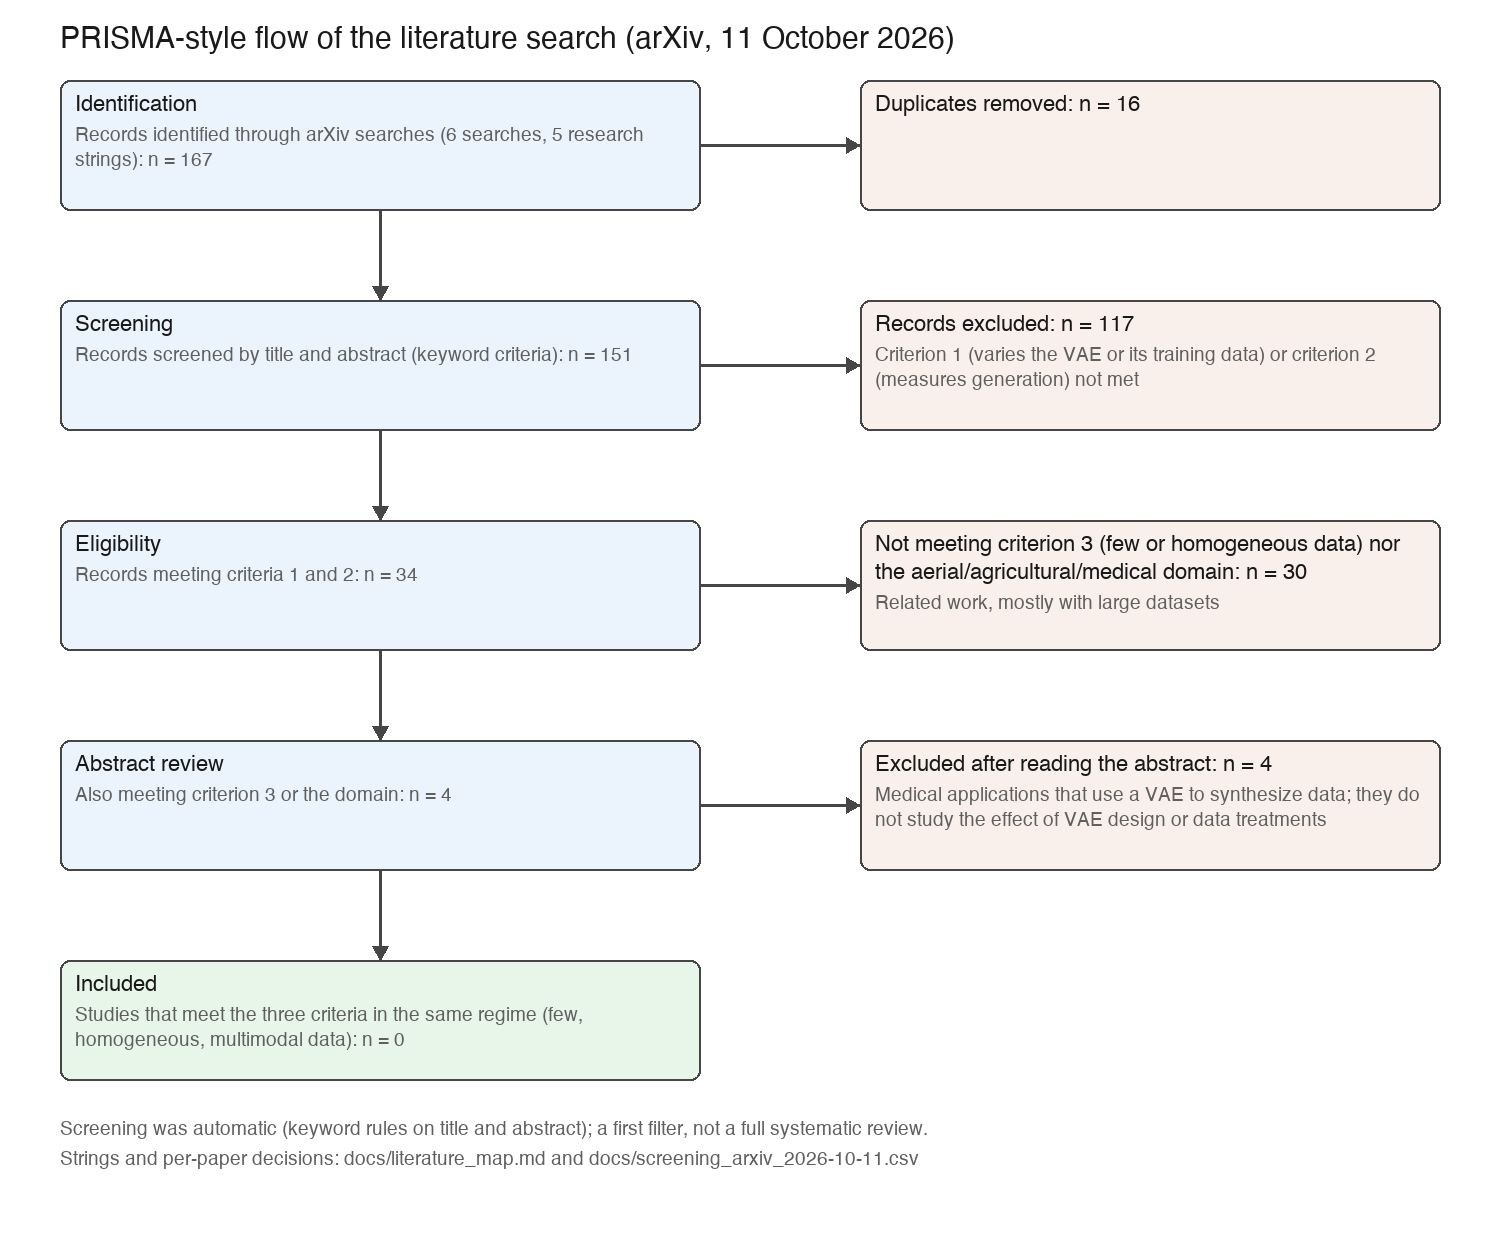
\includegraphics[width=0.95\textwidth]{Imagenes/prisma_arxiv.png}
\caption{PRISMA-style flow of the literature search on arXiv (11 October 2026). Screening was automatic, based on keyword rules over title and abstract.}
\label{fig:prisma}
\end{figure}

\textbf{Limitations.} Only arXiv was searched, the screening relied on keywords, and the search was not repeated by a second reviewer; it is a first systematic search and not a full systematic review.



%----------------------------------------------------------------------------------------
%	Capítulo 2
%----------------------------------------------------------------------------------------
\renewcommand{\baselinestretch}{1.5}

\chapter{Hypothesis and Objectives}

\section{Problem}

La generación de imágenes sintéticas con modelos de difusión latente se ha estudiado sobre todo con conjuntos de datos grandes y diversos. En agricultura de precisión, en cambio, los datos suelen ser pocos, homogéneos (las imágenes se parecen mucho entre sí: mismo cultivo, altura de vuelo y tipo de escena, con poca variabilidad) y, cada vez más, multimodales (cada imagen combina varias fuentes de información, por ejemplo color y profundidad). Este trabajo parte de un conjunto de 4\,908 imágenes aéreas de plantaciones de piña (resolución 960$\times$544), con una variante que añade un canal de profundidad monocular estimada.

Un modelo de difusión latente se entrena en dos etapas: un autoencoder variacional (VAE) comprime la imagen a un espacio latente (aquí, 4$\times$32$\times$32 para recortes de 256$\times$256) y un generador (DDPM o Flow Matching) aprende a producir latentes a partir de ruido. La calidad del espacio latente fija el techo de lo que el generador puede lograr, pero las decisiones sobre qué datos alimentan al VAE y cómo se estructura se toman hoy de forma manual y su efecto sobre la \emph{generación} no está claro. En particular, la literatura reciente señala que mejorar la reconstrucción de un VAE no implica mejorar la generación, pero esto se ha estudiado con grandes volúmenes de datos y no en un régimen de pocos datos homogéneos.

El problema que aborda esta propuesta es determinar cómo la variación de los datos de entrenamiento y de la estructura del VAE afecta la calidad de las imágenes aéreas de piña generadas mediante difusión latente, y a qué costo.

\section{Hypothesis}

Se plantean dos hipótesis, una sobre el efecto de manipular los datos y la estructura del VAE y otra sobre el límite de esa mejora:

\begin{enumerate}
  \item \textbf{Mejora.} Aplicar tratamientos a los datos de entrenamiento del VAE (aumento, enmascarado aleatorio, selección de imágenes y modalidad, con o sin canal de profundidad) y modificar su estructura (capa variacional y pérdida adversarial con un discriminador tipo GAN) mejorará el FID y el KID de las imágenes aéreas de piña generadas con modelos de difusión (DDPM y Flow Matching), en comparación con un VAE base sin tratamientos (entrenado solo con recortes aleatorios de 256$\times$256), sobre un conjunto de datos pequeño, homogéneo y multimodal.
  \item \textbf{Límite.} La mejora de la generación al acumular estos tratamientos y modificaciones presentará rendimientos decrecientes: existirá un punto a partir del cual aumentar la calidad de reconstrucción del VAE no reducirá significativamente el FID ni el KID.
\end{enumerate}

La primera hipótesis se refuta si ninguna combinación de tratamientos y modificaciones reduce el FID/KID de forma significativa respecto al VAE base; la segunda, si el FID/KID sigue reduciéndose significativamente en todos los escalones de la manipulación.

\section{Objectives}

\subsection{Main Objective}

Evaluar experimentalmente el efecto de variar los datos de entrenamiento y la estructura del VAE sobre la calidad de las imágenes aéreas de piña generadas mediante difusión latente, en un régimen de pocos datos homogéneos y multimodales.

\subsection{Specific Objectives}

\begin{enumerate}
  \item Implementar una línea base reproducible del pipeline VAE + generador (DDPM y Flow Matching), con una receta de entrenamiento controlada y verificada.
  \item Comparar tratamientos de los datos de entrada del VAE: aumento, enmascarado aleatorio, selección de imágenes y modalidad (RGB y RGB con profundidad).
  \item Comparar modificaciones estructurales del VAE: capa variacional, pérdida adversarial (GAN) y regularización.
  \item Analizar estadísticamente, con varias semillas, la relación entre la calidad de reconstrucción del VAE y la calidad de generación (FID/KID).
  \item Experimentar con un encoder auto-supervisado preentrenado (DINO) como espacio latente alternativo.
  \item Elaborar un artículo con los resultados del estudio.
\end{enumerate}

\subsection{Deliverables}

\begin{table}[h]
\centering
\small
\begin{tabular}{p{0.34\textwidth}p{0.58\textwidth}}
\hline
\textbf{Objetivo específico} & \textbf{Entregable} \\
\hline
1. Línea base reproducible & Informe de auditoría del pipeline y de la receta de entrenamiento corregida; código y configuraciones. \\
2. Efecto de los datos & Familia de VAEs entrenados con cada tratamiento de los datos; tabla comparativa de FID/KID y reconstrucción. \\
3. Efecto de la estructura & VAEs con capa variacional, GAN y regularización; análisis de su efecto sobre la reconstrucción y la generación. \\
4. Reconstrucción contra generación & Análisis estadístico (correlaciones, curvas, intervalos de confianza) con varias semillas. \\
5. Espacios latentes alternativos & Prototipo con un encoder auto-supervisado (DINO) y su comparación con el VAE base. \\
6. Artículo & Manuscrito con los resultados del estudio. \\
\hline
\end{tabular}
\caption{Entregables asociados a cada objetivo específico.}
\end{table}

\section{Research questions}

\begin{itemize}
  \item \textbf{RQ1.} ¿Cómo afecta la variación de los datos de entrenamiento del VAE (tratamientos: aumento, enmascarado, selección, modalidad) a la calidad de las imágenes generadas?
  \item \textbf{RQ2.} ¿Cómo afectan las modificaciones estructurales del VAE (capa variacional, GAN, regularización) a la calidad de las imágenes generadas?
  \item \textbf{RQ3.} ¿Se traduce una mejor reconstrucción del VAE en una mejor generación, o existe un punto a partir del cual deja de ayudar?
  \item \textbf{RQ4.} ¿Puede un encoder auto-supervisado preentrenado sustituir a un VAE entrenado desde cero en este régimen de datos?
\end{itemize}

\section{Scope and Limitations}

\subsection{Scope}

\begin{itemize}
  \item Un único conjunto de datos de imágenes aéreas de piña (4\,908 imágenes; 3\,536 para entrenamiento, 381 para validación y 346 para prueba), con recortes de 256$\times$256.
  \item VAE convolucional de espacio latente 4$\times$32$\times$32 y dos generadores: DDPM y Flow Matching, ambos con una U-Net convolucional sin atención.
  \item Calidad medida con FID y KID sobre imágenes generadas y un conjunto de referencia fijo; reconstrucción medida con MSE y PSNR.
  \item Núcleo del estudio: objetivos 1 a 4. Extensión, si el tiempo lo permite: objetivo 5.
  \item Extensión: la validación en otros dominios con conjuntos de datos pequeños y homogéneos, como las imágenes médicas, queda como extensión del estudio y no forma parte del núcleo.
\end{itemize}

\subsection{Limitations}

\begin{itemize}
  \item No se evalúa la utilidad de las imágenes sintéticas en una tarea posterior (por ejemplo, detección); se mide solo su calidad generativa.
  \item La profundidad es una estimación monocular relativa, no una medición de sensor.
  \item El número de semillas por condición está acotado por el costo de cómputo (unas 28 horas de GPU por entrenamiento).
  \item El FID se calcula con un número limitado de imágenes generadas (400), por lo que se acompaña de KID y de intervalos de confianza.
  \item Los resultados corresponden a un cultivo y a un conjunto de datos; su generalización a otros dominios no se evalúa.
\end{itemize}


%----------------------------------------------------------------------------------------
%	Capítulo 3
%----------------------------------------------------------------------------------------

\renewcommand{\baselinestretch}{1.5}

\chapter{Hypothesis and Objectives}

\section{Problem}

Latent diffusion models \cite{Rombach2022} compress each image with an autoencoder and run the diffusion process in the resulting latent space, which makes training far cheaper than diffusion in pixel space. Recent work on how to design that latent space has been carried out mostly on large benchmarks such as ImageNet \cite{Yao2025,Skorokhodov2025,Zheng2025}. In contrast, regional agricultural applications are characterized by small, homogeneous datasets, whereas most diffusion models are designed for massive and highly diverse ones \cite{Gonzalez2026}. Limited datasets and imbalanced sample distributions are a recurrent challenge in agricultural image analysis \cite{Hu2025}. Agricultural imagery is also increasingly multimodal, and latent diffusion models that jointly generate appearance and geometry from a shared latent space have been proposed \cite{Krishnan2025}.

The quality of the latent space matters for generation beyond reconstruction fidelity. Increasing the number of latent channels per position (the feature dimension per token) improves the reconstruction of the autoencoder but requires substantially larger diffusion models and more training to reach comparable generation \cite{Yao2025}; latent spaces with excessive high-frequency components hinder the diffusion process \cite{Skorokhodov2025}; and a recent systematic study reports that better reconstruction of the autoencoder (tokenizer) does not necessarily translate into better generation \cite{Zhong2026}. Under a limited training budget, a higher-dimensional latent space even degraded generation \cite{Sehwag2025}. Treatments of the training data such as random masking have also been used to learn better representations \cite{He2022} and tokenizers for diffusion \cite{Chen2025}.

This work starts from a set of 4,908 aerial images of pineapple plantations (resolution 960$\times$544), with a variant that adds an estimated monocular depth channel. A latent diffusion model is trained in two stages: a variational autoencoder (VAE) compresses the image into a latent space (here, 4$\times$32$\times$32 for 256$\times$256 crops) and a generator (DDPM or Flow Matching, FM) learns to produce latents from noise. In this setting, a continuous VAE latent space preserved crop structure where a discrete one failed \cite{Gonzalez2026}, but the choices of which data feed the VAE and how it is structured are usually made through manual experimentation \cite{Gonzalez2026}, without a systematic assessment of their effect on generation. Related questions have been studied with large datasets \cite{Yao2025,Skorokhodov2025,Zhong2026}, but, according to the literature search of October 2026 described in Chapter~II (Section~\ref{sec:litsearch}), the effect of data treatments and structural modifications of the VAE on generation has not been studied in a regime of few, homogeneous, and multimodal data. The closest work identified measured the effect of preprocessing on the generation quality of a latent diffusion model in a small medical cohort \cite{Fallah2026}, but it varied a single treatment, did not modify the structure of the VAE, and did not consider aerial, agricultural, or multimodal data.

The problem addressed by this proposal is to determine how varying the training data and the structure of the VAE affects the quality of aerial pineapple images generated through latent diffusion, and at what cost.

\section{Research Questions}

The problem motivates two research questions, which in turn motivate the hypothesis:

\begin{itemize}
  \item \textbf{RQ1.} What effect does each treatment of the training data of the VAE (augmentation, random masking, image selection, and modality) have on the quality of the images generated through latent diffusion, alone or in combination?
  \item \textbf{RQ2.} What effect does each structural modification of the VAE (variational output layer and adversarial loss) have on that quality, alone or in combination?
\end{itemize}

\section{Hypothesis}

\begin{center}
\begin{minipage}{0.92\textwidth}
\centering\itshape
Treatments of the training data and structural modifications of a variational autoencoder (VAE) produce measurable differences in the generation quality of latent generative models (Denoising Diffusion Probabilistic Model, DDPM, and Flow Matching, FM), as assessed by the Fr\'echet Inception Distance (FID) and the Kernel Inception Distance (KID), when trained on a small, homogeneous UAV dataset.
\end{minipage}
\end{center}

The treatments considered are data augmentation, random masking, image selection, and depth modality (RGB, or RGB with estimated depth); the modifications are a variational output layer and an adversarial loss with a GAN-style discriminator. The difference is always measured with respect to a base VAE trained only with random crops. The effect of each treatment and modification is estimated separately, and their interactions are explored as a secondary analysis.

The hypothesis is supported if, across seeds, at least one treatment or modification has a statistically significant effect on the FID, with the KID pointing in the same direction (analysis of variance, with correction for multiple comparisons). It is evaluated first with DDPM, and the effects found are then checked with FM. It is refuted if the effect of every treatment and modification is equivalent to zero within a margin set from the noise measured in Stage 0 (equivalence tests); if neither holds, the evidence is inconclusive for the factors involved.

\section{Objectives}

\subsection{Main Objective}

To experimentally evaluate the effect of varying the training data and the structure of the VAE on the quality of aerial pineapple images generated through latent diffusion, in a regime of few, homogeneous, and multimodal data.

\subsection{Specific Objectives}

\begin{enumerate}
  \item To implement a reproducible baseline of the VAE + generator pipeline (DDPM and FM), with a controlled and verified training recipe.
  \item To compare treatments of the VAE input data: augmentation, random masking, image selection, and modality (RGB and RGB with depth).
  \item To compare structural modifications of the VAE: variational output layer and adversarial loss (GAN).
  \item To statistically analyze, with several seeds, the relationship between the reconstruction quality of the VAE and the generation quality (FID/KID).
  \item To explore the feasibility of using a pretrained self-supervised encoder (DINO) as an alternative latent space representation for image generation under limited training data, and to compare its performance with the VAE baseline.
  \item To write a paper with the results of the study.
\end{enumerate}

\subsection{Deliverables}

\begin{table}[h]
\centering
\small
\begin{tabular}{p{0.34\textwidth}p{0.58\textwidth}}
\hline
\textbf{Specific objective} & \textbf{Deliverable} \\
\hline
1. Reproducible baseline & Audit report of the pipeline and of the corrected training recipe; code and configurations. \\
2. Effect of the data & Family of VAEs trained with each data treatment; comparative table of FID/KID and reconstruction. \\
3. Effect of the structure & VAEs with variational output layer and GAN; analysis of their effect on reconstruction and generation. \\
4. Reconstruction versus generation & Statistical analysis (correlations, curves, confidence intervals) with several seeds. \\
5. Alternative latent spaces & Prototype with a self-supervised encoder (DINO) and its comparison with the base VAE. \\
6. Paper & Manuscript with the results of the study. \\
\hline
\end{tabular}
\caption{Deliverables associated with each specific objective.}
\end{table}

\section{Scope and Limitations}

\subsection{Scope}

\begin{itemize}
  \item A single dataset of aerial pineapple images from a plantation in Costa Rica (4,908 frames of 960$\times$544 pixels, reduced from 1\,920$\times$1\,088; 3,536 for training, 381 for validation, and 346 for testing, split by blocks of capture), with 256$\times$256 crops. It was chosen because it represents the regime of interest, with few and homogeneous images of one field, an estimated depth channel, and bounding boxes of the plants, and because it belongs to the line of work of the research group on pineapple drone imagery \cite{XieLi2024,Fallas2023,XieLi2025VAE,Gonzalez2026}.
  \item The frames were captured top-down at an altitude of two meters. This is lower than the 30 and 70~m compared in a recent study of corn detection \cite{Barboza2025}, and close to the 3 to 7~m and 5~m of very-low-altitude studies of wheat plant density \cite{Jin2017} and spruce seedlings \cite{Lopatin2023}. Altitude balances spatial resolution against coverage and flight time \cite{Guess2025}; at two meters each frame shows only a few plants (3.6 annotated boxes per frame on average), so the data require more flight time per area, a cost consistent with the scarcity this work addresses.
  \item A convolutional VAE with a 4$\times$32$\times$32 latent space and two generators: DDPM and FM, both with a convolutional U-Net without attention.
  \item The weight of the KL regularization of the VAE is kept fixed in all runs ($\beta=0.001$ for the latent); it is not an experimental factor and its effect is not evaluated.
  \item Quality measured with FID and KID on generated images and a fixed reference set; reconstruction measured with MSE and PSNR.
  \item Core of the study: objectives 1 to 4. Extension, if time permits: objective 5.
  \item Extension: validation on a second UAV crop, or in other domains with small, homogeneous datasets, such as medical images, is left as an extension of the study and is not part of the core.
\end{itemize}

\subsection{Limitations}

\begin{itemize}
  \item The usefulness of the synthetic images in a downstream task (for example, detection or counting) is not evaluated, and labeling the generated images is left as future work; only their generative quality is measured.
  \item Depth is a relative monocular estimate, not a sensor measurement.
  \item The KL weight of the latent is fixed at $\beta=0.001$, the value that balanced reconstruction and latent structure in earlier work on this plantation \cite{XieLi2025VAE}, and not a value selected for generation; the KL weight of the output layer is also fixed. A different value could change the results, and the effect of these weights is left as future work.
  \item The FID and the KID are computed on the RGB channels, so the depth channel of the generated images is not evaluated, and they do not detect the memorization of training images \cite{Stein2023}.
  \item The number of seeds per condition is bounded by the computational cost (about 26 GPU hours per training run).
  \item FID is computed with a finite number of generated images, so it is biased and noisy; it is accompanied by KID and confidence intervals, and the number of images is chosen in Stage~0 (Chapter~IV).
  \item The results correspond to one crop and one dataset; their generalization to a second crop or to other domains is not evaluated.
  \item The data preparation, the input of the VAE, and the evaluation protocol differ from those of the work this proposal builds on \cite{Gonzalez2026}, so the values of FID and KID are not directly comparable with the Fr\'echet Distance reported there.
\end{itemize}

%-----------------
%	Capítulo 4
%-----------------

\renewcommand{\baselinestretch}{1.5}

\chapter{Workplan}

 \section{Tasks}
 \section{Schedule}




%-----------------
%	Capítulo 5
%-----------------

\renewcommand{\baselinestretch}{1.5}

\chapter{Initial Results}

% Sources: docs/ of this repository and the audit report (propuesta/Informe_avance_reunion.html in Latent-Diffusion).

\section{Audit of the Training Pipeline}

% TODO: the seven problems found, with the evidence for each (learning-rate scheduler, best-checkpoint criterion, gradient clipping, decoder noise, sigma of the latent, in-place decoder operation, uncertainty).

\section{Generation Quality of the Retrained Models}

% TODO: FID and KID table (original VAE and new VAE, DDPM and Flow Matching, best and final checkpoint) and the attribution caveat: the new VAE changes three things at once.

\section{Reconstruction Pilots with Masking}

% TODO: masked-input VAEs (25 and 50 percent) against the control, when the runs finish.


%-----------------
%	Capítulo 6
%-----------------

\renewcommand{\baselinestretch}{1.5}

\chapter{Workplan}

This chapter organizes the work needed to carry out the experimental design of Chapter~IV. The work is planned by calendar month (Figure~\ref{fig:gantt}): the corrections of this proposal take place from November 2026 to January 2027, the research phase starts in February 2027, and the delivery of the thesis is expected about October 2027. The periods are estimates.

\section{Tasks}

\subsection{Proposal and Literature}

\begin{itemize}
  \item Finish the research proposal: related work, the state of the art, and the corrections requested by the advisor.
  \item Keep the literature search up to date with the strings and sources of Chapter~II, and read in full the works that are closest to the hypothesis.
\end{itemize}

\subsection{Code and Infrastructure}

\begin{itemize}
  \item Add a switch that turns off the variational output layer of the decoder, so that factor E can be tested.
  \item Make every replicate use its own seed for the VAE and for the generator, and record the seeds.
  \item Integrate masking and image selection in the training of the VAE as factors that can be switched on and off from the configuration.
  \item Write the evaluation scripts (FID, KID, PSNR, SSIM, and the FID of the reconstructions) so that every run is evaluated in the same way.
  \item Sample the generated images in batches, so that the number of images chosen in Stage~0 is affordable.
  \item Generate the fractional design, check its aliasing, and randomize the order of the runs; write the analysis script in R.
  \item Define the workflow of the cluster: at most four jobs at a time, evaluation after each run, and archiving or deletion of checkpoints to respect the storage quota.
\end{itemize}

\subsection{Stage 0: Noise and Convergence}

Train five replicates of the base cell, check that the VAE converges with the fixed number of epochs, estimate the standard deviation of the FID between independent runs, set the margin of the equivalence tests, and choose the number of generated images $N$ by comparing the sampling noise of the FID with the variation between runs (Chapter~IV).

\subsection{Stage 1: Screening}

Run the $2^{6-2}$ design with DDPM and three replicates per cell (48 runs; the period reserved for this stage leaves room for up to five replicates), evaluate every run, and analyze the results with the analysis of variance, the equivalence tests, and the correlation between reconstruction and generation.

\subsection{Stage 2: Refinement}

Choose the factors that showed an effect and study them with a full factorial design and more levels, resolving the interactions that were aliased in Stage 1.

\subsection{Stage 3: Confirmation with Flow Matching}

Repeat the factors that mattered with Flow Matching (FM) in a small full factorial design, to check that the effect does not depend on the generator.

\subsection{Optional Work}

\begin{itemize}
  \item If time permits, prototype a pretrained self-supervised encoder (DINO) as an alternative latent space (objective 5).
  \item If an opportunity arises, a month, flexible within the schedule, could be used to apply the findings to a second crop with UAV imagery, for example during a research exchange in Osnabr\"uck; this is not part of the objectives, and the runs of the cluster can continue during it.
\end{itemize}

\subsection{Paper and Thesis}

Write a paper with the results of the study (objective 6) and write the thesis. The drafting starts in February with the introduction, the related work, and the method, which this proposal already contains, and the results are added as each stage ends.

\section{Schedule}

Table~\ref{tab:schedule} shows the phases with their period and the computing time they need. The computing times come from the budget of Chapter~IV (about 26 hours per generator and about 14 hours per VAE trained from scratch, with four jobs in parallel); the durations include time for the queue of the cluster and for runs that must be repeated.

\begin{table}[H]
\centering
\small
\begin{tabular}{p{0.30\textwidth}p{0.17\textwidth}p{0.24\textwidth}p{0.21\textwidth}}
\hline
\textbf{Phase} & \textbf{Period (2027)} & \textbf{Computing} & \textbf{Output} \\
\hline
Proposal and corrections & Nov 2026 to Jan & -- & Approved proposal \\
Code and infrastructure & Feb to Mar & -- & Switch, seeds, batched sampling, scripts, design \\
Stage 0: noise and convergence & Apr & about 200 GPU hours (4 days), plus the sampling for $N$ & Standard deviation, epochs, margin, $N$ \\
Stage 1: screening & May to Jun & about 1\,900 GPU hours (20 days); room for five replicates & 48 evaluated runs \\
Analysis of Stage 1 & Jul & -- & Factors that matter \\
Stage 2: refinement & Jul to Aug & about 700 GPU hours (8 days)\textsuperscript{a} & Effects and interactions \\
Stage 3: confirmation & Aug to Sep & about 420 GPU hours (5 days) & Check with FM \\
Final analysis and thesis & Sep to Oct & -- & Thesis \\
Paper and thesis drafting & Feb to Sep (parallel) & -- & Paper draft \\
Optional: DINO extension & Jul to Sep & -- & Prototype \\
Optional: stay in Osnabr\"uck & one month, Apr to Sep & -- & Cross-crop check \\
\hline
\end{tabular}
\caption{Phases of the work. \textsuperscript{a}Estimate that depends on the factors selected in Stage 1. The drafting of the paper starts in February and the results are added as they appear; the stay in Osnabr\"uck is a flexible month.}
\label{tab:schedule}
\end{table}

\begin{figure}[H]
\centering
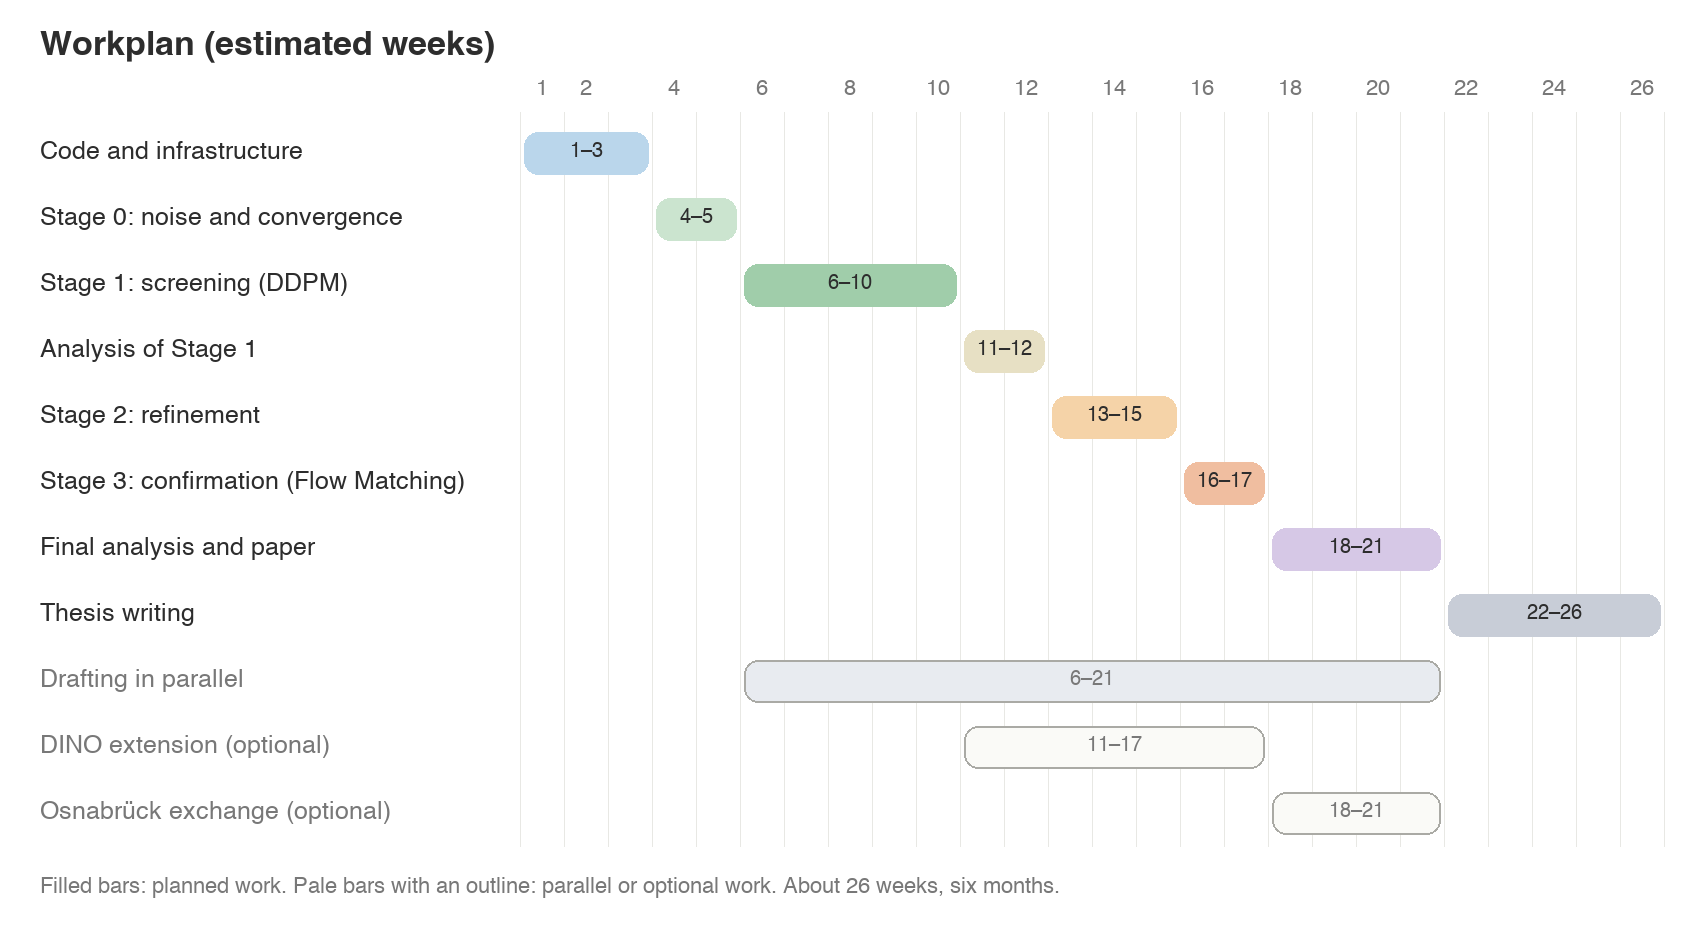
\includegraphics[width=0.95\textwidth]{Imagenes/gantt_workplan.png}
\caption{Workplan by calendar month. Filled bars are planned work; pale bars with an outline are parallel or optional work.}
\label{fig:gantt}
\end{figure}

The research phase lasts about eight months, from February to October 2027. The main risks are the availability of the cluster, which limits the work to four jobs at a time, the storage quota, and runs that fail or diverge. Stage 1 is scheduled for May and June because its runs need little attention; if the standard deviation measured in Stage 0 is larger than expected, the number of replicates is increased up to five, which that period allows, and, if more were needed, the schedule would be extended.



%-----------------
%	Conclusiones
%-----------------

% \renewcommand{\baselinestretch}{1.5}
\chapter*{\centering \large CONCLUSIONS} % No numerado, centrado
\addcontentsline{toc}{chapter}{CONCLUSIONS} 
\markboth{CONCLUSIONS}{CONCLUSIONS} % encabezado


 %Se agregan las conclusiones (no son necesarias en la propuesta, confirmado por el asesor). Para activarlas, quitar el % inicial.


%----------------------------------------------------------------------------------------
%	BIBLIOGRAFIA
%----------------------------------------------------------
%------------------------------
\newpage
\bibliography{TFC1/biblio} %Se agrega la bibliografia


%----------------------------------------------------------------------------------------
%	Anexos
%----------------------------------------------------------------------------------------
% Anexos desactivados: la plantilla traía 'ANNEX 1, 2, 3' vacíos que saldrían en el PDF. Para usarlos (por ejemplo, declaración de uso de IA), quitar los % siguientes.
% \appendix

% \renewcommand{\appendixname}{ANNEXES}% annexes
% \chapter*{\appendixname}
% \addcontentsline{toc}{chapter}{ANNEX} 
% \markboth{ANNEX}{ANNEX} % encabezado

%  \thispagestyle{empty}
 



% \textbf{ANNEX 1} 

%  \textbf{ANNEX 2} 
 
%  \textbf{ANNEX 3} 
 


%  \phantomsection
\end{document} 


